
\documentclass[12pt]{article}

\usepackage{sbc-template}
\usepackage{caption}
\usepackage{float}
\usepackage{graphicx,url}

\usepackage[brazilian]{babel}   
\usepackage[T1]{fontenc}
\usepackage[utf8]{inputenc} 
\usepackage{multicol}
\usepackage{multirow}
\usepackage{graphicx,url}
\usepackage{amsmath,amssymb,amsfonts}
\usepackage{algorithmic}
\usepackage{textcomp}
\usepackage{url}
\usepackage{enumerate}
\usepackage{multirow}
\usepackage{soul}
\usepackage{verbatim}
\usepackage[table,xcdraw]{xcolor}
\usepackage[shortlabels]{enumitem}
\usepackage{scalefnt}
\usepackage{comment}
\usepackage{lscape}
\usepackage{fancyhdr}
\usepackage[super]{nth}
\usepackage{booktabs}
\usepackage{longtable}

\DeclareUnicodeCharacter{0327}{\c{}}
\DeclareUnicodeCharacter{0301}{\'{}}
\tolerance=1
\emergencystretch=\maxdimen
\hyphenpenalty=10000
\hbadness=10000

\title{Uma Revisão Sistemática sobre o Gargalo de Von Neumann: Estratégias na Hierarquia de Memória Cache e Armazenamento Secundário \\
\medskip
\small{
    \textit{A Systematic Review on the Von Neumann Bottleneck: Strategies in Cache Memory Hierarchy and Secondary Storage}
}
}

\author{Anderson Vicente de Freitas\inst{1}, André Hércules Gonçalves da Silva Pereira\inst{1},\\ Walter Felipe Dos Santos\inst{1} }

\address{Colegiado De Ciencia Da Computação \\
Universidade Federal do Vale do São Francisco (UNIVASF) -- Campus Salgueiro \\
Salgueiro -- CEP: 56.000-000 -- PE -- Brasil
}


\begin{document} 

\maketitle

\thispagestyle{plain}

\begin{abstract}
The von Neumann bottleneck is a limitation on the transfer rate between the
processor and the main memory of a computer, in which the same transfer line
is used for both instructions and data, a problem aggravated by the uneven
evolution of the two components. A bibliographic review was therefore carried
out using textbooks, teaching material and articles, selected and filtered
according to strict criteria. The concepts found were organized into a
taxonomy and represented in diagrams and tables, and the average memory
access time model was described using hypothetical values. Multilevel
caches, write policies, SSDs as HDD caches and virtual memory, with the risk
of \textit{thrashing}, are some of the strategies used to mitigate the von
Neumann bottleneck. Future projections point to in-memory computing and
hybrid systems to overcome the problem.
\end{abstract}

\keywords{Von Neumann bottleneck, Memory hierarchy, Cache memory, Secondary
storage, Computer architecture.}

\begin{resumo}
O Gargalo de von Neumann é uma limitação na taxa de transferência entre o
processador e a memória principal de um computador, no qual a mesma linha de
transferência é utilizada tanto para instruções quanto para dados, problema
agravado também pela evolução descompassada entre os dois componentes.
Assim, foi realizada uma pesquisa bibliográfica através de livros-texto,
material didático, artigos, selecionados e filtrados segundo critérios
rígidos. Os conceitos encontrados foram organizados na forma de uma
taxonomia, representados em diagramas e tabelas, e o modelo
de tempo médio de acesso foi descrito usando valores hipotéticos. Caches multinível,
políticas de escrita, SSD como cache para HDD e memória virtual com o risco de
\textit{thrashing} são algumas estratégias utilizadas para amenizar o
Gargalo de von Neumann. Projeções futuras indicam computação em memória e
sistemas híbridos para superar o problema.
\end{resumo}

\palavraschave{Gargalo de von Neumann, Hierarquia de memória, Memória cache,
Armazenamento secundário, Arquitetura de computadores.}

\section{Introdução} \label{sec:introducao}

A computação moderna tem origem em sua primeira geração na década de 1940, com a criação do ENIAC (Electronic Numerical Integrator and Computer), considerado o primeiro computador digital eletrônico de propósito geral do mundo, que tinha como objetivo realizar cálculos complexos  mais rápido que cálculos humanos com enfoque bélico na Segunda Guerra Mundial \cite{stallings2010}. Sua programação, porém, era exaustiva por ser feita manualmente, por meio da reconexão de cabos e do ajuste de chaves \cite{miletto2014}. Esse processo exaustivo mais tarde seria otimizado com a criação do conceito de \textit{Programa Armazenado}: no qual instruções e dados passaram a ficar na mesma memória, isso permitiu que as tarefas pudessem ser mudadas apenas rodando um software diferente \cite{stallings2010}. Posteriormente, em 1945, John von Neumann iniciou o projeto do EDVAC (Electronic Discrete Variable Computer), essa ideia deu origem à Arquitetura de von Neumann: composta por memória principal, unidade lógica e aritmética (ULA), unidade de controle (UC), dispositivos de entrada e dispositivos de saída. Essa arquitetura é praticamente a base da construção da maioria dos computadores atuais \cite{tanenbaum2013}. Esse modelo apresenta, contudo, uma limitação central,  conhecida como o Gargalo de von Neumann: como instruções e dados utilizam o mesmo caminho de comunicação entre a CPU e a memória principal, faz com que a taxa de transferência entre esses dois componentes seja limitada, o que consequentemente pode afetar o desempenho geral da máquina. O problema se agrava à medida que os processadores evoluíram em ritmo muito superior em relação à memória ao longo dos anos \cite{couto2017}.

Este artigo apresenta uma revisão bibliográfica das estratégias da
hierarquia de memória que atenuam o gargalo de von Neumann, da memória cache até o armazenamento secundário. Como contribuição,
propõe tabelas comparativas e um diagrama da hierarquia, elaborados e adaptados pelos
autores, além de discutir os \textit{trade-offs} de latência, custo e capacidade.
A Seção~\ref{sec:metodologia} descreve a Metodologia de Pesquisa; a
Seção~\ref{sec:taxonomia}, a Taxonomia e a Sistematização Teórica; a
Seção~\ref{sec:analise}, a Análise Crítica e discussões sobre os Gargalos Arquiteturais; e a Seção~\ref{sec:conclusao}
contém as Considerações Finais.

\section{Metodologia} \label{sec:metodologia}

Este trabalho trata de uma revisão bibliográfica de natureza teórica e analítica referente à área de Arquitetura e Organização de Computadores. Por ter caráter estritamente bibliográfico, não há experimentação empírica no projeto: baseia-se exclusivamente na leitura, comparação e síntese da literatura, tendo como objetivo responder à seguinte questão norteadora: quais são as estratégias que minimizam o Gargalo de von Neumann e quais são os \textit{trade-offs} envolvidos? 

Os materiais de referência foram coletados e selecionados por meio do Google Acadêmico e da bibliografia da disciplina. Foram incluídos livros-texto \cite{stallings2010, tanenbaum2013, hennessy2017}, materiais didáticos \cite{miletto2014, oliveira2019, couto2017}, além de artigos relacionados à hierarquia de memória, cache, armazenamento secundário, gerência de memória e sites sobre o contexto atual do gargalo de von Neumann \cite{maues2025, ferreira2015, santos2015, souza2023, hess2025}. Foram incluídas as fontes que tratam explicitamente da arquitetura de von Neumann, da organização da memória, da cache ou do armazenamento secundário, enquanto foram excluídos os textos que mencionam a arquitetura de von Neumann sem entrar em detalhes sobre suas técnicas e funcionamento.

Para a análise, foram seguidas as seguintes etapas: (i) seleção do material segundo os critérios mencionados; (ii) criação de uma taxonomia dos conceitos presentes nos materiais (Seção~\ref{sec:taxonomia}), desde a origem do gargalo até as estratégias de cache e de armazenamento secundário; (iii) demonstração do impacto do gargalo na latência usando o modelo do tempo médio de acesso (Seção~\ref{sec:amat}), cujos valores apresentados são hipotéticos e ilustram ordens de grandeza, uma vez que não há medição empírica direta; e (iv) níveis da hierarquia de memória e comparação entre as estratégias e(Figura~\ref{fig:hierarquia_memoria} e~\ref{tab:estrategias_mitigacao}). Além disso, é feita uma discussão crítica sobre latência, custo, capacidade e os \textit{trade-offs} envolvidos no processo de mitigação do Gargalo de von Neumann (Seção~\ref{sec:analise}). 

O texto foi redigido pelos autores. Ferramentas de inteligência artificial generativa foram utilizadas apenas para checagem gramatical do documento e para auxiliar no código \LaTeX, conforme definido nas diretrizes da disciplina.

\section{Taxonomia e Sistematização Teórica} \label{sec:taxonomia}

\subsection{A Arquitetura de Von Neumann e a Origem do Gargalo} \label{sec:origem}
A arquitetura de von Neumann baseia-se em três princípios: dados e instruções ficam em uma única memória de leitura e escrita; o conteúdo dessa memória é endereçável por posição, independentemente do tipo de dado; e a execução é sequencial, salvo desvio explícito \cite{stallings2010}. Seus componentes são a memória principal, os dispositivos de entrada e saída e a CPU, formada pela ULA, pela unidade de controle e pelos registradores \cite{couto2017, tanenbaum2013} (Figura~\ref{fig:von_neumann}). A unidade de controle busca as instruções uma a uma e coordena sua execução, no ciclo de busca, decodificação e execução \cite{couto2017}.

Como instruções e dados trafegam pelo mesmo canal entre a CPU e a memória, a taxa de transferência desse canal se limita a taxa com que o processador consegue operar, e a CPU precisa esperar pelos dados. Esse é o Gargalo de von Neumann, termo atribuído a John Backus em sua palestra do Prêmio Turing de 1977 \cite{couto2017}. O problema se agravou porque a velocidade da CPU e o tamanho da memória evoluíram em ritmo superior ao da taxa de transferência entre eles \cite{couto2017}. Uma forma de reduzi-lo é inserir uma cache entre a CPU e a memória principal e separar as caches de instruções e de dados, o que se chama arquitetura Harvard modificada \cite{couto2017}.

\begin{figure}[H]
\centering
\caption{Máquina original de von Neumann.}
\label{fig:von_neumann}
\vspace{6pt}

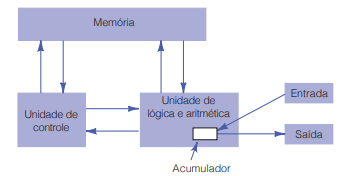
\includegraphics[width=0.55\textwidth]{Figuras/fig_von_neumann.png}

\vspace{6pt}
\small{\textit{Fonte:} \cite{tanenbaum2013}}
\end{figure}

\subsection{Hierarquia de Memória e Princípio da Localidade}
\label{sec:hierarquia}
Para conciliar custo, capacidade e velocidade, a memória é organizada em uma hierarquia, tradicionalmente representada como uma pirâmide que abrange desde os níveis mais rápidos e restritos até os de maior capacidade e menor velocidade, sendo composta por registradores, memória cache, memória principal e armazenamento secundário.

\begin{figure}[H]
\centering
\caption{Hierarquia de memória.}
\label{fig:hierarquia_memoria}
\vspace{6pt}

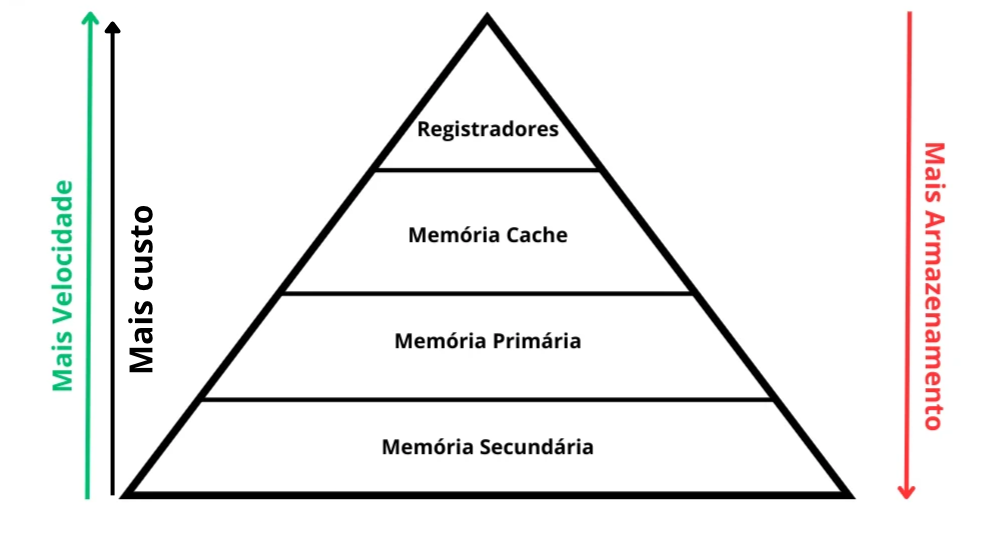
\includegraphics[width=0.55\textwidth]{Figuras/fig_hierarquia_memoria.png}

\vspace{6pt}
\small{\textit{Fonte:} adaptado pelos autores(2026) de~\cite{maues2025}}
\end{figure}

Os níveis dessa hierarquia e suas principais características funcionais e tecnológicas são descritas da seqguinte forma por \cite{maues2025}:

\begin{itemize}
    \item \textbf{Registradores}: localizados no interior da CPU, constituem o nível mais rápido, de menor latência e de capacidade mais restrita da hierarquia, sendo responsáveis por armazenar operandos e instruções imediatamente utilizados pelo processador.
    \item \textbf{Memória Cache}: atua como um nível intermediário entre os registradores e a memória principal (RAM). Sua principal função é armazenar dados e instruções acessados com maior frequência para reduzir a latência de acesso.
    \item \textbf{Memória Principal (RAM)}: memória do tipo volátil e de capacidade intermediária que mantém as informações de forma temporária durante a execução dos programas e do sistema operacional. Apresenta menor velocidade em comparação aos níveis superiores, contudo oferece capacidade substancialmente maior a um custo inferior por bit.
    \item \textbf{Memória Secundária}: composta por dispositivos não voláteis como discos rígidos (HDD) e unidades de estado sólido (SSD), caracteriza-se pela alta capacidade de armazenamento e pelo baixo custo. É responsável pela retenção permanente de dados, arquivos e do sistema operacional.
\end{itemize}
O funcionamento eficiente dessa hierarquia apoia-se no Princípio da Localidade de Referência, que define a tendência de um processador acessar o mesmo conjunto de locais de memória. Esse princípio subdivide-se em:
\begin{itemize}
    \item \textbf{Localidade Temporal}: refere-se à tendência de um dado ou instrução recentemente acessado ser requisitado novamente em um curto intervalo de tempo. Exemplos incluem funções, métodos, laços de repetição, contadores e variáveis modificadas com frequência \cite{ferreira2015}.
    \item \textbf{Localidade Espacial}: corresponde à tendência de itens armazenados em endereços de memória adjacentes ao item recém-acessado serem requisitados em seguida. Nessa categoria encontram-se partes procedurais e sequenciais do programa, além de estruturas de dados como vetores, matrizes e listas \cite{ferreira2015}.
\end{itemize}

\subsection{Funcionamento e Estratégias na Memória Cache}  \label{sec:amat}
Sem cache, cada ciclo de instrução exigiria ao menos um acesso à memória principal e, como a DRAM é mais lenta que a execução da instrução, o processador ficaria ocioso \cite{ferreira2015}. A cache atenua esse descompasso armazenando cópias das instruções e dos dados mais usados \cite{stallings2010, ferreira2015}. Quando a CPU requisita uma palavra, ocorre um acerto (\textit{cache hit}) se ela está em alguma linha da cache, sendo entregue ao processador em um tempo $T_{acerto}$; caso contrário, ocorre uma falha (\textit{cache miss}), e o dado é buscado nos níveis inferiores, com uma penalidade $P_{falha}$ correspondente à latência da DRAM e ao trânsito no barramento. Para reduzir falhas futuras, a transferência ocorre em blocos de palavras adjacentes, aproveitando a localidade espacial \cite{stallings2010, ferreira2015}.

O efeito da cache pode ser medido pelo tempo médio de acesso à memória (AMAT) que, com base no modelo de dois níveis de ~\cite{stallings2010}, é dado por:
\begin{equation}
T_{med} = T_{acerto} + (1 - h) \times P_{falha}
\end{equation}
, em que $h$ é a taxa de acerto e $(1 - h)$ é a taxa de falhas. Com valores hipotéticos $T_{acerto} = 5\text{ ns}$ (ordem de grandeza de uma cache L2), $P_{falha} = 60\text{ ns}$ e $h = 0,95$, tem-se $T_{med} = 5 + 0,05 \times 60 = 8\text{ ns}$. A penalidade de falha é doze vezes o tempo de acerto, mas o tempo médio fica próximo ao da cache; ainda assim, as falhas, que ocorrem em apenas $5\%$ dos acessos, respondem por 3 dos 8 ns ($37,5\%$).

Os projetos de cache combinam algumas estratégias. Na hierarquia multinível (L1, L2 e L3), a L1, interna ao processador, é a menor e mais rápida; a L2 é intermediária; e a L3, compartilhada entre os núcleos, é a última barreira antes da DRAM, de modo que a capacidade cresce para os níveis inferiores, enquanto a velocidade e o custo por bit crescem para os superiores \cite{stallings2010, ferreira2015}. Nas caches separadas, a divisão da L1 em instruções (L1I) e dados (L1D) elimina a disputa entre a busca de instruções e a unidade de execução no pipeline, concretizando a arquitetura Harvard modificada da Seção~\ref{sec:origem}, embora a cache unificada tenda a ter taxa de acerto maior para o mesmo tamanho \cite{stallings2010}.

Quanto ao mapeamento de endereços, o mapeamento direto associa cada bloco a uma única linha, sendo simples e barato, mas sujeito a faltas por conflito; o totalmente associativo permite qualquer linha, sem conflitos, mas exige comparar as etiquetas de todas elas; e o associativo por conjuntos de $k$ vias combina simplicidade e flexibilidade \cite{stallings2010}. Na política de escrita, o \textit{write-through} grava na DRAM a cada escrita, mantendo os dois níveis consistentes, mas gera tráfego que pode saturar o barramento; o \textit{write-back} grava apenas na cache, marca a linha com um bit de modificação (\textit{dirty bit}) e atualiza a DRAM só quando o bloco é descartado \cite{stallings2010}. Ferreira \cite{ferreira2015} relata ganhos de até $15\%$ em processadores Cyrix e de cerca de $30\%$ em processadores IBM com o \textit{write-back}. Por fim, quando o conjunto está cheio, algoritmos como LRU (descarta o bloco menos recentemente usado, preservando a localidade temporal), FIFO ou aleatório escolhem o bloco a ser substituído \cite{stallings2010}.

\subsection{Estratégias no Armazenamento Secundário} 
\label{sec:secundario}
Em geral, o armazenamento secundário apresenta latência bem superior à das memórias voláteis, por depender de meios físicos para a gravação de dados \cite{oliveira2019, stallings2010}. Os HDDs são os principais armazenadores de longo prazo por terem um baixo custo e grande capacidade. Porém, para ler um dado, o braço de leitura precisa ser posicionado para pesquisa (\textit{seek time}), que varia entre 4 e 10 ms, e o disco deve girar até que o setor seja acessado (latência rotacional), que varia entre 3 e 7 ms \cite{santos2015}. Essa característica torna o acesso custoso e gera um tempo mais lento do que o acesso à DRAM. Assim, uma das grandes dificuldades de projeto é lidar com E/S.

Uma estratégia é o uso de memória virtual: a partir da necessidade de mais memória RAM do que a disponível por parte dos programas, o sistema operacional divide o espaço de endereçamento em páginas de tamanho fixo. A página é carregada a partir do disco, conforme necessário, para uma área chamada \textit{swap} \cite{souza2023}. Esse processo corre o risco de gerar o \textit{thrashing}, que ocorre quando o conjunto de trabalho (\textit{working set}) é maior que a RAM e, consequentemente, a maior parte dos ciclos é consumida na transferência de páginas entre o disco e a memória, o que prejudica o sistema \cite{souza2023}. 

\begin{figure}[H]
\centering
\caption{Tabela comparativa das estratégias de mitigação do Gargalo de Von Neumann}
\label{tab:estrategias_mitigacao}
\vspace{6pt}
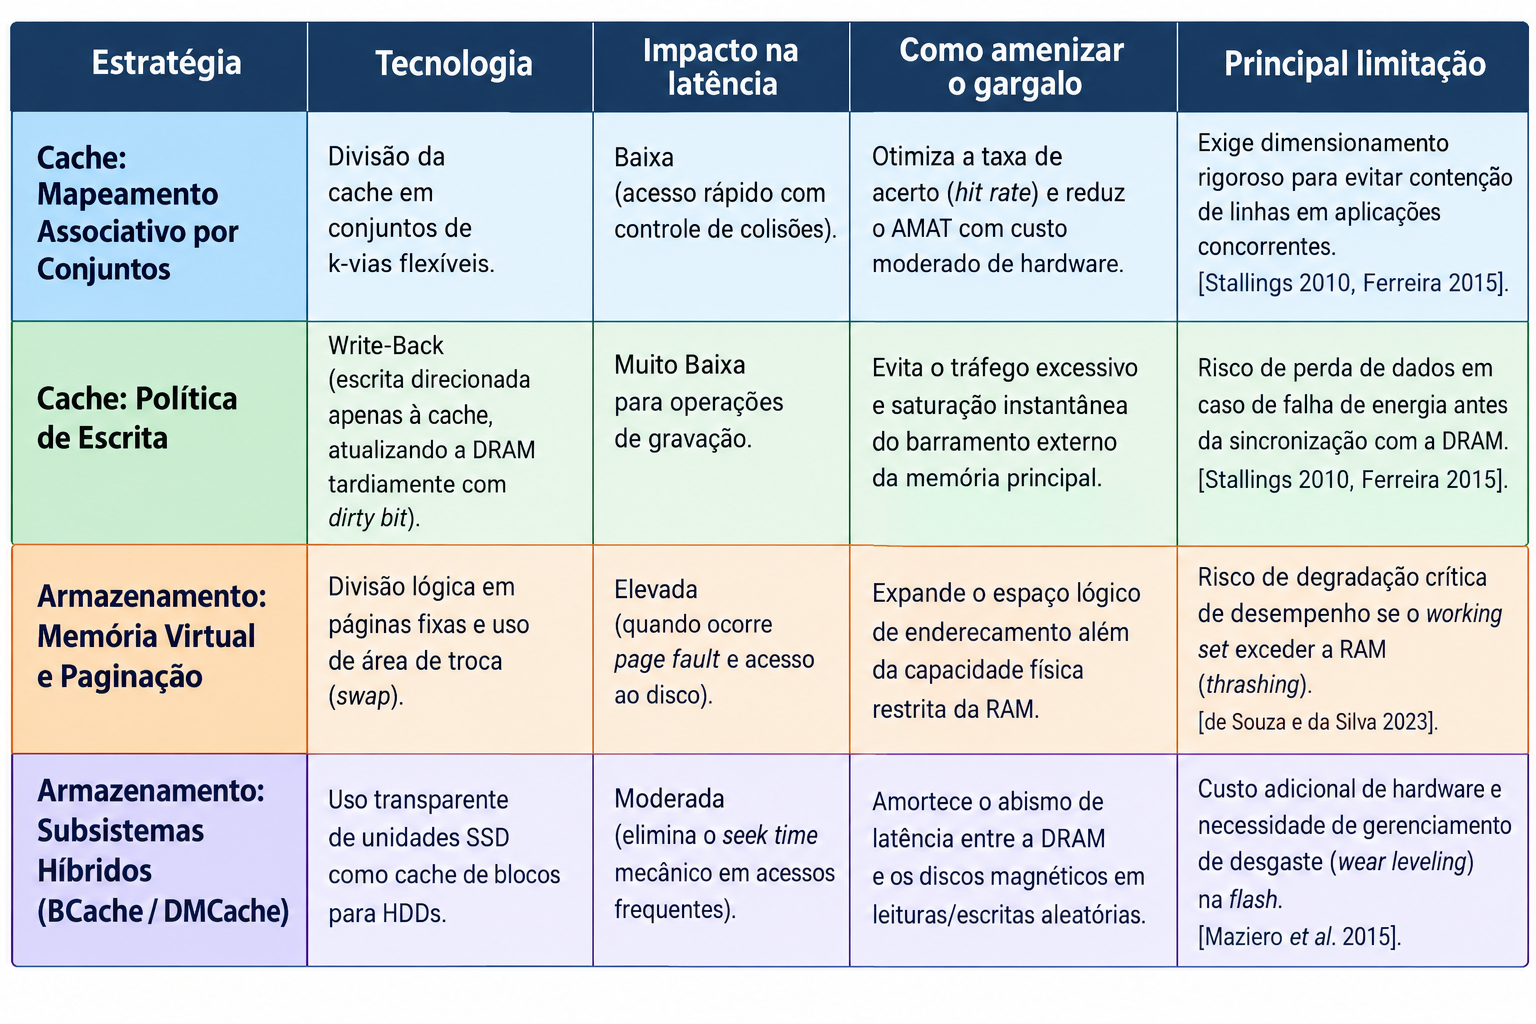
\includegraphics[width=0.95\textwidth]{Tabelas/tab_estrategias_mitigacao.png}

\vspace{6pt}
\small{\textit{Fonte:} Elaborado pelos autores (2026), com base em \cite{stallings2010, ferreira2015, souza2023, santos2015}.}
\end{figure}

Os SSDs são mais rápidos que os HDDs pois utilizam memória NAND \textit{flash}. Porém, não são vistos para substituir os HDDs para conjuntos massivos de dados, pois possuem custo mais alto por gigabyte, além de uma capacidade menor. Uma alternativa é utilizar o SSD como uma cache transparente dos dados mais acessados do HDD \cite{santos2015}. No Linux, existem soluções como \textit{BCache} e \textit{DMCache}. O \textit{BCache} trabalha na camada de blocos, independente do sistema de arquivos, e possui a vantagem de permitir acesso aleatório e ignorar solicitações estritamente sequenciais. O \textit{DMCache} utiliza o \textit{device-mapper} e exige partições dedicadas; além disso, permite três modos de escrita: \textit{write-back} (apenas na cache), \textit{write-through} (na cache e no dispositivo subjacente ao mesmo tempo) e \textit{write-around} (diretamente no dispositivo subjacente) \cite{santos2015}. A Figura~\ref{tab:estrategias_mitigacao} compara as estratégias de armazenamento secundário com as de cache.

\section{Análise Crítica e Gargalos Arquiteturais} \label{sec:analise}

\subsection{O Descompasso Físico e os Limites da Escalabilidade} \label{sec:limitacoes}
Com o avanço das tecnologias de processadores, as memórias principais não acompanharam este avanço. Isto resulta em casos nos quais a CPU entra em modo de espera (wait time) para aguardar a chegada dos dados \cite{stallings2010, tanenbaum2013}. O problema ocorre devido ao fato de que a DRAM armazena informações em capacitores, que ao receberem um bit, perdem carga ao longo do tempo, exigindo ciclos periódicos de atualização (\textit{refresh}). Já a SRAM da cache utiliza flip-flop para armazenamento, não precisa realizar refresh, porém requer mais transistores para armazenar um bit, resultando em maior custo de implementação e menor densidade de integração \cite{stallings2010}. Desta forma, a memória cache é rápida, porém com pequena capacidade e alto custo, sendo a memória principal de maior capacidade, porém mais lenta. (Figura~\ref{tab:tradeoffs_hierarquia}).

O aumento da frequência de operação também fez surgir limites físicos: a partir de 2001, o aquecimento causado pela redução espacial dos transistores não podia ser dissipado utilizando-se refrigeração convencional. Isto fez com que o aumento do clock se tornasse difícil, o que levou os fabricantes a resolverem este impasse utilizando-se de processadores multicore \cite{ferreira2015}. Com vários núcleos, o barramento tende a se tornar um ponto de contenção arquitetural. Para contornar essa situação, foi utilizada uma cache L3 compartilhada entre todos os núcleos (microarquitetura Nehalem). Esta cache atua inclusivamente sobre as caches L1 e L2 de cada núcleo, e evita que cada núcleo verifique a cache privada dos outros núcleos, o que aumenta consideravelmente o rendimento do sistema como um todo \cite{ferreira2015}.

\subsection{Síntese dos Trade-Offs da Hierarquia de Memória}
\label{sec:tradeoffs}
A Figura~\ref{tab:tradeoffs_hierarquia} apresenta uma síntese comparativa dos níveis que compõem a hierarquia de memória, destacando as ordens de grandeza típicas de latência, as capacidades ilustrativas e os principais compromissos de projeto associados a cada tecnologia.

\begin{figure}[H]
\centering
\caption{Tabela comparativa dos níveis da hierarquia de memória e trade-offs arquiteturais}
\label{tab:tradeoffs_hierarquia}
\vspace{6pt}

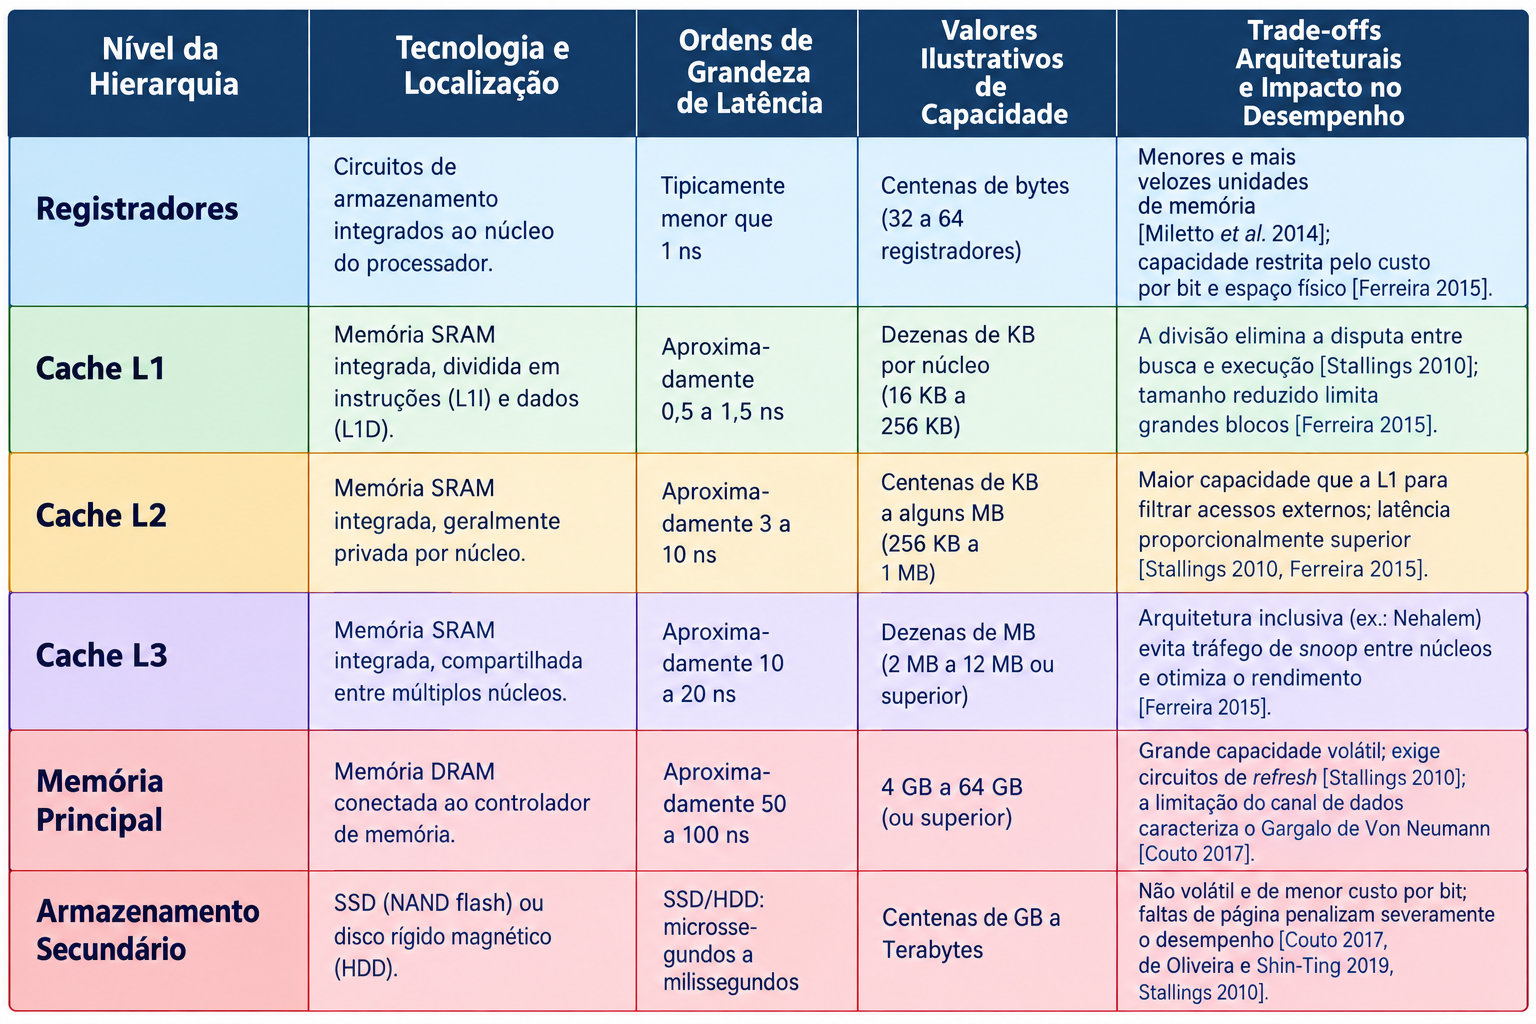
\includegraphics[width=0.95\textwidth]{Tabelas/tab_tradeoffs_hierarquia.png}

\vspace{6pt}
\small{\textit{Fonte:} Elaborado pelos autores (2026) com base em \cite{couto2017, ferreira2015, hennessy2017, miletto2014, oliveira2019, stallings2010}.A capacidade das memórias e as ordens de grandeza de latência por nível são baseadas em \cite{hennessy2017}.}
\end{figure}

Em síntese, a Figura~\ref{tab:tradeoffs_hierarquia} evidencia o compromisso fundamental da hierarquia: os níveis superiores (registradores e caches SRAM) priorizam velocidade e baixa latência, enquanto os inferiores (DRAM e armazenamento secundário) oferecem alta capacidade e persistência a um custo por bit viável. Como, em geral, quanto maior a capacidade de um nível, menor sua velocidade de acesso, o desempenho computacional global depende diretamente da eficiência dos mecanismos de mitigação do gargalo de von Neumann ao longo de toda a estrutura.

\section{Considerações Finais} \label{sec:conclusao}

Neste artigo, foram revistas as principais estratégias existentes na hierarquia de memória para minimizar o Gargalo de von Neumann. A discrepância entre a velocidade da CPU e a latência da DRAM, amplificada pela barreira térmica do \textit{clock} e pela contenção no barramento em sistemas \textit{multicore} \cite{ferreira2015, tanenbaum2013}, é contornada pelo uso de caches multinível, que aproveitam a localidade para diminuir o tempo médio de acesso por meio de políticas de escrita como o \textit{write-back}, o\textit{write-through} e \textit{write-around} \cite{stallings2010, ferreira2015}, além do uso de SSDs e subsistemas de cache de bloco no armazenamento secundário para atenuar a diferença de latência em relação aos HDDs \cite{santos2015}. Contudo, ressalta-se que esse gargalo não é eliminado, mas apenas reduzido.

As tendências futuras na computação, impulsionadas principalmente pela inteligência artificial, revelam os limites das estratégias atuais. O processo de carregar os bilhões de pesos de um modelo a partir da memória é constante, e a transferência de dados consome a maior parte da energia, enquanto o cálculo representa apenas cerca de $10\%$ da carga, segundo pesquisadores da IBM \cite{hess2025}. Para combater esse cenário, surgiram novas soluções: a computação em memória utiliza a memória de mudança de fase (\textit{Phase Change Memory} -- PCM) para armazenar os pesos do modelo na resistividade do material, minimizando a transferência de dados. No entanto, devido à baixa durabilidade da PCM, essa abordagem limita-se à execução de modelos previamente treinados em GPUs. Outras inovações incluem a computação próxima à memória, como no processador IBM NorthPole, que dota cada núcleo de sua própria memória SRAM, e a óptica co-embalada, que estende a largura de banda da fibra óptica até a borda do chip \cite{hess2025}. Como a arquitetura de von Neumann continua fundamental para a computação de propósito geral e para operações de alta precisão, projeta-se o advento de sistemas híbridos que combinem processadores de von Neumann e não von Neumann \cite{hess2025}. 

\bibliographystyle{sbc}
\bibliography{Referencias/referencias}

\end{document}
